\documentclass{article}
\usepackage{longtable}
\usepackage{graphicx}  % For adding logos/images
\usepackage{tikz}
\usepackage{fancyhdr}  % For header/footer customization
\usepackage{amsmath}   % For math formatting
\usepackage{geometry}  % For page margin adjustments
\geometry{a4paper, margin=1in}

\usepackage{background}  % To include background patterns (optional)


\definecolor{lightgray}{gray}{0.96}
\definecolor{mintgreen}{rgb}{0.88, 1.0, 0.88}  % Define mint green color
\pagecolor{lightgray}  % Set the entire page to mint green

% \backgroundsetup{
%   scale=1,
%   color=black,
%   opacity=0.1,        % Set opacity to make the pattern subtle
%   angle=0,
%   position=current page.center,
%   contents={
%     \begin{tikzpicture}[remember picture, overlay]
%       \foreach \x in {-15,-14,...,15} {
%         \foreach \y in {-20,-20,...,20} {
%           \node at (\x, \y) {
%             \begin{tikzpicture}
%               % Hexagon drawing with 60-degree angles
%               \draw[fill=lightgray!40] (90:0.2) -- (150:0.2) -- (210:0.2) -- (270:0.2) -- (330:0.2) -- (30:0.2) -- cycle;
%             \end{tikzpicture}
%           };
%         }
%       }
%     \end{tikzpicture}
%   }
% }


\title{\Huge \textbf{Aarkus Intelligence: \\ Vision for Blockchain Data Analytics}}
\author{
  \textbf{Harsh Gupta} \\
  Founder, Aarkus Intelligence \\
  \texttt{harsh@aarkusintelligence.com}
}
\date{\today}

\pagestyle{fancy}
\fancyhf{}
\fancyhead[L]{Aarkus Intelligence Whitepaper}
\fancyhead[R]{\thepage}
\fancyfoot[C]{Draft 1}

% \usetikzlibrary{shapes.geometric, arrows.meta}

% \tikzstyle{block} = [rectangle, rounded corners, minimum width=3cm, minimum height=1cm, text centered, draw=black, fill=blue!20]
% \tikzstyle{arrow} = [thick,-{Stealth[round]}]
% \tikzstyle{circleblock} = [circle, minimum width=1.5cm, text centered, draw=black, fill=green!20]


\begin{document}

\maketitle
\thispagestyle{empty} % To remove page number on the title page

\begin{abstract}
\textit{
The abstract provides an overview of Aarkus Intelligence, focusing on our mission to empower traders with blockchain-based insights and innovative data analysis tools. This document outlines the architecture, utility, and vision behind Aarkus Intelligence, a platform for smarter decision-making in crypto trading.
}
\end{abstract}

\tableofcontents

\newpage

\section{Introduction}
The explosive growth of blockchain technology has introduced an unprecedented influx of data, creating both opportunities and challenges for traders and investors. With the rise of decentralized finance (DeFi), cryptocurrency trading, and non-fungible tokens (NFTs), blockchain has become a cornerstone for digital assets. However, this same expansion has overwhelmed traders with vast, unstructured data, making it difficult to extract actionable insights.

% \begin{tikzpicture}[node distance=2cm]

%   % Main central block (Aarkus Intelligence)
%   \node (aarkus) [circleblock] {Aarkus Intelligence};
  
%   % Key Features (Real-time Data Capture, AI-Powered Insights, Automated Trade Analysis)
%   \node (data) [block, above left of=aarkus, xshift=-1cm, yshift=1cm] {Real-time Data Capture};
%   \node (ai) [block, above right of=aarkus, xshift=1cm, yshift=1cm] {AI-Powered Insights};
%   \node (trade) [block, below of=aarkus, yshift=-1cm] {Automated Trade Analysis};
  
%   % Blockchain, Wallets, and Assets representations
%   \node (blockchain) [block, below left of=trade, xshift=-1cm, yshift=-1cm] {Blockchain Networks};
%   \node (wallets) [block, below of=trade, yshift=-1cm] {Wallets};
%   \node (assets) [block, below right of=trade, xshift=1cm, yshift=-1cm] {Assets};
  
%   % Arrows connecting the central block to the features
%   \draw [arrow] (aarkus) -- (data);
%   \draw [arrow] (aarkus) -- (ai);
%   \draw [arrow] (aarkus) -- (trade);
  
%   % Arrows connecting the features to Blockchain, Wallets, Assets
%   \draw [arrow] (trade) -- (blockchain);
%   \draw [arrow] (trade) -- (wallets);
%   \draw [arrow] (trade) -- (assets);
  
%   \end{tikzpicture}

At its core, Aarkus Intelligence revolutionizes the trading landscape by providing an automated solution that enables traders to visualize, track, and analyze every trade they make across any blockchain without any manual intervention. By seamlessly capturing and processing blockchain trade data, Aarkus delivers real-time performance insights and trend analysis, empowering traders to make data-driven decisions. Whether managing a single wallet or multiple assets across various chains, Aarkus ensures precision in tracking every trade. Powered by AI, the platform transforms raw blockchain data into strategic intelligence, helping traders uncover patterns, predict trends, and optimize their strategies in a fast-paced, ever-evolving market.

By eliminating the need for manual tracking, Aarkus significantly reduces the complexity of analyzing blockchain activity, allowing traders to focus on optimizing their strategies. The platform’s AI-powered insights provide a deeper understanding of wallet behavior, market trends, and asset movements, offering traders a clear edge in an increasingly competitive market.

Additionally, with rising cryptocurrency scams and fraud, Aarkus Intelligence integrates advanced security analytics to detect anomalies and provide actionable insights to protect traders from malicious activities. The result is a comprehensive tool that not only enhances performance but also ensures the safety and integrity of every trade.

\section{Market Opportunity for Aarkus Intelligence}

Aarkus Intelligence targets two key customer segments: \textbf{ardent crypto traders (B2C)} and \textbf{blockchain-based companies with native crypto tokens (B2B)}. Each segment benefits from blockchain transaction data analytics and wallet intelligence in different ways. This market is evolving rapidly due to the increased adoption of blockchain technology, the growth of decentralized finance (DeFi), and the rise of cryptocurrencies globally.

\subsection{1. Ardent Crypto Traders (B2C)}

This segment consists of highly active and knowledgeable individuals who engage in frequent trading of digital assets. These traders rely on \textbf{real-time blockchain transaction data} to optimize their trading strategies. The need for wallet intelligence—providing insights into on-chain activities, wallet behaviors, and market trends—is essential for traders to make informed decisions.

In 2024, over \textbf{420 million people globally own cryptocurrency}, and the number of crypto transactions is growing exponentially \cite{DemandSage, Cognitive}. As crypto markets are decentralized, traders require tools that give them a competitive edge, such as \textbf{real-time analytics}, wallet monitoring, and predictive insights. Millennials and Gen Z dominate this space, accounting for \textbf{70\% of crypto traders} \cite{DemandSage}. These traders are looking for platforms that provide transparent, secure, and data-driven insights into wallets and transactions, helping them identify trends and opportunities.

However, the rapid growth of the crypto space has also led to a rise in crypto-related scams and fraud. In 2022 alone, crypto scams resulted in losses exceeding \textbf{\$4.3 billion}, impacting both individual traders and companies alike \cite{Fortune}. Common scams, such as rug pulls, phishing attacks, and market manipulations, exploit the decentralized and often anonymous nature of blockchain transactions. These malicious activities not only harm traders but also erode trust in the broader blockchain ecosystem. Ardent crypto traders, who operate in fast-moving markets, often lack the tools to detect suspicious wallet behaviors or track unusual token movements.

\begin{figure}[h!]
  \centering
  \includegraphics[width=0.8\textwidth]{wallet_growth_trend.png}  % Placeholder for wallet growth trend graph
  \caption{Projected Growth of Crypto Wallet Users (2023-2029)}
  \label{fig:wallet_growth}
\end{figure}

\begin{longtable}{|p{4cm}|p{8cm}|}
\hline
\textbf{Statistic} & \textbf{Value} \\
\hline
Global Crypto Wallet Owners (2024) & 420 million \\
\hline
Crypto Fraud Losses (2022) & \$4.3 billion \\
\hline
Dominance of Millennials/Gen Z in Crypto Trading & 70\% \\
\hline
\caption{Crypto Market Overview (2022-2024)}
\end{longtable}

\subsection{2. Blockchain Projects \& Crypto Companies (B2B)}

Blockchain-based companies that operate with their native crypto tokens—such as DeFi projects, tokenized platforms, and blockchain infrastructure providers—constitute the B2B customer base for Aarkus Intelligence. These companies rely heavily on \textbf{blockchain transaction data} to manage liquidity, monitor user activity, and ensure regulatory compliance. With over \textbf{81\% of the top 100 public companies} adopting blockchain technology, the need for data analytics platforms that track wallet behavior and transaction flows is growing \cite{DemandSage}.

The total global blockchain market size is expected to expand at a \textbf{CAGR of 66.2\%} from 2024 to 2031 \cite{Cognitive}. Companies that launch their tokens require comprehensive intelligence to understand how tokens are used, traded, and held across different wallets. For these companies, insights into \textbf{token circulation}, \textbf{whale activities}, and potential \textbf{market manipulation} are crucial for maintaining market integrity and trust.

By offering real-time data analytics on wallets and transactions, Aarkus Intelligence provides these companies with the ability to make \textbf{data-driven decisions}, manage their token economies more efficiently, and maintain transparent relationships with their communities. As the blockchain ecosystem rapidly evolves and blockchain projects proliferate globally, there is a growing demand for platforms that integrate \textbf{blockchain data analysis}, \textbf{security monitoring}, and \textbf{wallet intelligence} to maintain token stability and optimize ecosystem operations.

% \begin{figure}[h!]
%   \centering
%   \includegraphics[width=0.8\textwidth]{defi_growth.png}  % Placeholder for DeFi market growth diagram
%   \caption{Growth of DeFi Market and Tokenized Ecosystems (2020-2024)}
%   \label{fig:defi_growth}
% \end{figure}

\begin{longtable}{|p{4cm}|p{8cm}|}
\hline
\textbf{Metric} & \textbf{Value} \\
\hline
Global Blockchain Market CAGR (2024-2031) & 66.2\% \\
\hline
Companies Using Blockchain (2024) & 81\% of top 100 companies \\
\hline
\caption{Blockchain Market and Adoption Metrics}
\end{longtable}

\subsection{Market Growth Drivers}

The market growth for blockchain analytics and wallet intelligence is driven by several key factors:
\begin{itemize}
    \item \textbf{Adoption of Blockchain by Large Enterprises}: Companies worldwide are integrating blockchain technology, driving the need for sophisticated data analytics solutions.
    \item \textbf{Rising Usage of Digital Tokens and DeFi}: DeFi and tokenized ecosystems are expanding rapidly, with the total value locked in DeFi projects surpassing \$200 billion in 2022.
    \item \textbf{Demand for Real-Time Data Analytics}: The increasing complexity of blockchain transactions and the need for real-time decision-making are pushing demand for platforms like Aarkus Intelligence.
\end{itemize}

% \begin{figure}[h!]
%   \centering
%   \includegraphics[width=0.8\textwidth]{market_drivers.png}  % Placeholder for market growth drivers graph
%   \caption{Key Market Growth Drivers (2022-2030)}
%   \label{fig:market_drivers}
% \end{figure}

\subsection{Who Will Use Aarkus Intelligence?}

Aarkus Intelligence will be used by two primary groups:
\begin{itemize}
    \item \textbf{Active Crypto Traders}: Individuals who trade frequently on decentralized platforms and need real-time insights to optimize their trading strategies.
    \item \textbf{Blockchain Projects and Tokenized Ecosystems}: Organizations with native tokens that require wallet monitoring, transaction analytics, and liquidity management tools.
\end{itemize}

\section{Vision \& Mission}
Describe the long-term vision and mission of Aarkus Intelligence.

\section{The Aarkus Intelligence Platform}
At the core of Aarkus Intelligence lies its unique ability to deliver a comprehensive and detailed representation of every transaction across any blockchain. This capability allows traders not only to visualize their trades in real time but also to have a precise and clear understanding of the transaction flow, significantly enhancing decision-making processes.

\subsection{Transactions: The Core of Trading}
In the blockchain ecosystem, transactions represent the atomic unit of value exchange. A transaction contains crucial information such as sender and recipient addresses, the asset being transferred, and associated transaction fees. Understanding these components is fundamental to accurate trade representation.

\begin{longtable}{|c|c|c|c|c|c|}
\hline
\textbf{Component} & \textbf{Description} & \textbf{Example Value} \\
\hline
Transaction Hash & Unique ID for the transaction & 0x123abc... \\
\hline
Block Number & Block where the transaction was confirmed & 120034 \\
\hline
Sender Address & Wallet initiating the transaction & 0xabc123... \\
\hline
Recipient Address & Wallet receiving the asset & 0xdef456... \\
\hline
Asset & The asset being transferred & ETH \\
\hline
Transaction Value & Amount of asset being transferred & 2 ETH \\
\hline
Gas Fee & Fee paid for processing the transaction & 0.01 ETH \\
\hline
\end{longtable}

Below is a simple representation of a transaction between 2 entities. The tokens that were exchanged, the time it happened and the transaction fees involved in the process.

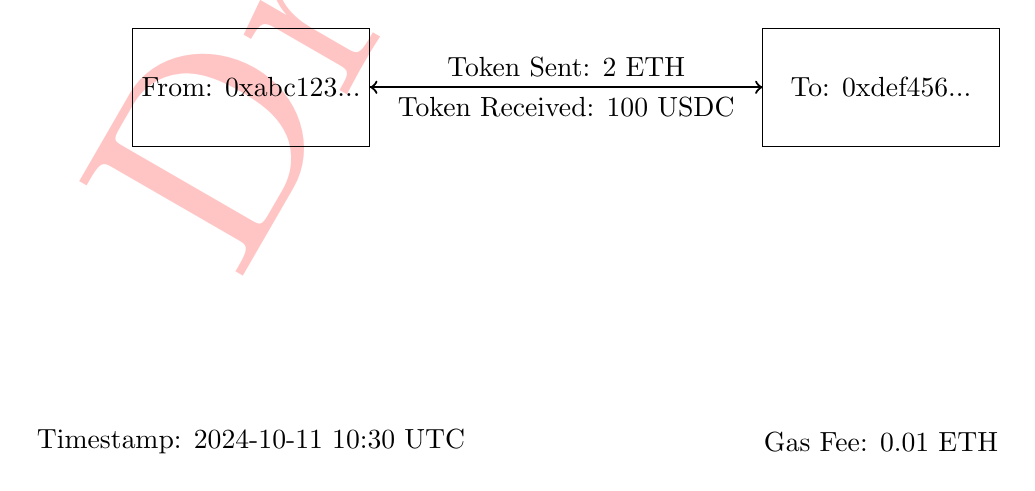
\begin{tikzpicture}[node distance=3cm, auto]

  % Define the transaction details
  \node (from) [rectangle, draw, text centered, minimum height=1.5cm, minimum width=3cm] {From: 0xabc123...};
  \node (to) [rectangle, draw, right of=from, xshift=5cm, text centered, minimum height=1.5cm, minimum width=3cm] {To: 0xdef456...};

  % Arrows representing token sent out and token received in
  \draw[->, thick] (from) -- (to) node[midway, above] {Token Sent: 2 ETH};
  \draw[<-, thick] (from) -- (to) node[midway, below] {Token Received: 100 USDC};

  % Timestamp and gas fee annotations
  \node (timestamp) [below of=from, yshift=-1.5cm] {Timestamp: 2024-10-11 10:30 UTC};
  \node (gasfee) [below of=to, yshift=-1.5cm] {Gas Fee: 0.01 ETH};

\end{tikzpicture}
\subsection{Transaction Flow and Portfolio Impact}


\begin{figure}[h!]
  \centering
  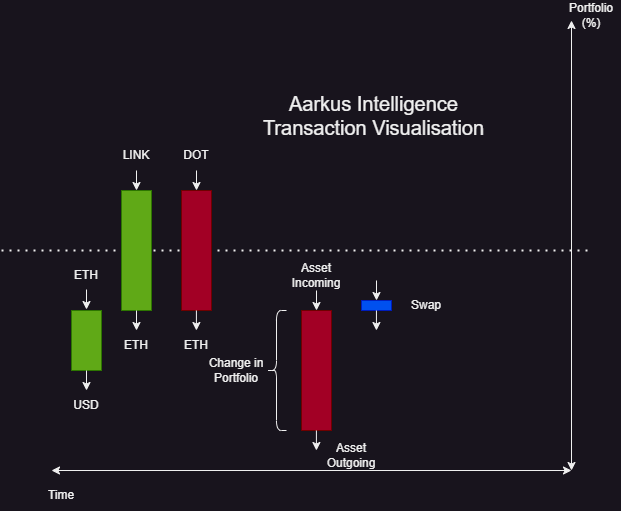
\includegraphics[width=0.8\textwidth]{TransactionVisualisation.png}  % Replace with your image file
  \caption{Aarkus Intelligence Transaction Visualization. The image above demonstrates how assets flow between addresses, showing tokens sent out, received, timestamp, and gas fees.}
  \label{fig:transaction_visualization}
\end{figure}

The visualization above illustrates how different blockchain transactions impact a portfolio over time. Let us break down the key elements of this diagram and explain it in terms of transaction and trade flow.

\subsubsection*{Key Elements of the Diagram}

\paragraph{X-Axis (Time):}
This represents the timeline over which various trades and transactions are performed. As time progresses from left to right, different asset movements occur in the portfolio.

\paragraph{Y-Axis (Portfolio Change):}
This represents the percentage change in the portfolio based on the incoming and outgoing assets. As trades occur, the portfolio either gains or loses value, which is reflected on this axis.

\subsubsection*{Transaction Flow:}

The diagram captures multiple trades happening over time:
\begin{itemize}
    \item \textbf{USD to ETH}: The initial trade where USD is converted into ETH, represented by the green bar. This shows a positive increase in the portfolio as ETH is acquired.
    \item \textbf{ETH to LINK}: The next trade where ETH is used to purchase LINK, represented by another green bar, indicating an increase in the portfolio’s value with the acquisition of LINK.
    \item \textbf{ETH to DOT}: Another trade follows, where ETH is converted into DOT, which is represented by the red bar, indicating a reduction in the ETH holdings and a corresponding addition of DOT to the portfolio.
\end{itemize}

\subsubsection*{Change in Portfolio:}
The change in portfolio is represented visually by the difference between incoming and outgoing assets. The green bars represent assets coming into the portfolio (increasing the portfolio’s value), while red bars represent assets leaving the portfolio (reducing its value).

\subsubsection*{Asset Incoming and Outgoing:}
In the middle of the diagram, the incoming and outgoing assets are highlighted side-by-side, showing the transaction flow. The incoming asset (in green) shows an asset being added to the portfolio, while the outgoing asset (in red) shows an asset being swapped or traded out of the portfolio.

\subsubsection*{Swap:}
The blue rectangle labeled \textbf{Swap} indicates an event where two assets are exchanged, such as swapping ETH for DOT. This swap impacts the portfolio's value, but the diagram emphasizes that it is a direct asset swap rather than a sale or acquisition.

\subsubsection*{Interpretation:}

\paragraph{Portfolio Over Time:}
The diagram highlights the sequential flow of transactions over time. As time progresses, the trader moves assets within their portfolio through different trades. Starting with USD, they purchase ETH, then trade some ETH for LINK, and finally use the remaining ETH to purchase DOT.

\paragraph{Impact on Portfolio:}
The green bars (gains) and red bars (losses) visually represent the flow of assets into and out of the portfolio. The portfolio gains ETH, which then gets partially converted into LINK, with the remaining ETH being converted into DOT.

\paragraph{Chained Transaction Visualization:}
This representation is ideal for illustrating chained transactions, where the output of one trade (e.g., ETH acquired from USD) becomes the input for another trade (e.g., ETH used to buy LINK and DOT). The cumulative effect on the portfolio is clearly visualized through the sequence of incoming and outgoing asset transactions.
\subsection{Trades: An Abstraction Over Transactions}
While transactions represent the building blocks of blockchain activity, trades are abstractions that bundle multiple transactions. A trade wraps around one or more transactions and brings additional contextual information, including strategy and status. Below is the structured table format for a trade.

\begin{table}[h!]
  \centering
  \begin{tabular}{|p{4cm}|p{8cm}|p{4cm}|}
  \hline
  \textbf{Parameter}        & \textbf{Description}                                & \textbf{Example}                     \\
  \hline
  Principle            & The principal asset involved in the trade      & 500 USDC                        \\
  \hline
  Time Invested        & Duration from trade initiation to completion   & 3 days                          \\
  \hline
  Transaction          & The transactions that constitute the trade     & USD/ETH, ETH/LINK               \\
  \hline
  Trade Type           & Type of trade (spot, margin, etc.)             & Spot Trade                      \\
  \hline
  PnL                  & Profit or Loss realized from the trade         & \$50                            \\
  \hline
  Trade Status         & Current state of the trade (open/closed)       & Closed                          \\
  \hline
  Trade Name           & A label to identify the trade                  & ETH Investment                  \\
  \hline
  Associated Strategy  & The strategy being applied (HODL, swing, etc.) & Swing Trading                   \\
  \hline
  Chained Trade        & Any subsequent trades linked to this trade     & ETH $\rightarrow$ LINK          \\
  \hline
  Visualization Option & Graphical representation of the trade          & Candlestick chart               \\
  \hline
  \end{tabular}
  \caption{Trade Parameters}
  \end{table}
  
For example, buying ETH with USD is one transaction, and using that ETH to purchase LINK is another. A trade combines these steps into a coherent strategy.

\textbf{Example:}
\begin{itemize}
    \item \textbf{Trade 1}: USD $\rightarrow$ ETH (0.25 ETH bought for 500 USD)
    \item \textbf{Trade 2}: ETH $\rightarrow$ LINK (0.1 ETH used to buy LINK)
    \item Remaining 0.15 ETH stays in the open USD/ETH trade.
\end{itemize}

The trades, based on these transactions, can be visualized as follows:

\scriptsize % Reduce the font size further
% Reduce table width with p{<width>} in longtable
\begin{longtable}{|p{1cm}|p{1.2cm}|p{1.2cm}|p{1.2cm}|p{1.2cm}|p{1.5cm}|p{1.5cm}|p{1.2cm}|p{1.2cm}|p{1.5cm}|}
\hline
\textbf{Trade ID} & \textbf{Pair} & \textbf{Entry Asset} & \textbf{Exit Asset} & \textbf{Amount} & \textbf{Price at Entry} & \textbf{Price at Exit} & \textbf{Status} & \textbf{Profit/Loss} & \textbf{Timestamp} \\
\hline
1 & USD/ETH & USD & ETH & 0.15 ETH & \$2000/ETH & N/A & Open & N/A & 2024-10-11 10:30 UTC \\
\hline
1 & USD/ETH & USD & ETH & 0.1 ETH & \$2000/ETH & \$2200/ETH & Closed & \$20 & 2024-10-11 11:00 UTC \\
\hline
2 & ETH/LINK & ETH & LINK & 0.1 ETH & \$2200/ETH & N/A & Open & N/A & 2024-10-11 11:00 UTC \\
\hline
\caption{Trade Tracking}
\end{longtable}
\normalsize % Return to normal font size
\subsection{Chained Transactions}

A chained transaction is a series of linked transactions where the output of one transaction becomes the input for another. In the context of Aarkus Intelligence, we can track these trades, showing both open and closed positions as well as the corresponding profits or losses.

Let’s consider the scenario where 500 USDC is used to purchase 0.25 ETH at a rate of \$2000/ETH. Afterward, a portion of that ETH (0.1 ETH) is used to buy LINK at a rate of \$7 per LINK. The USD/ETH trade remains partially open with 0.15 ETH.

\subsubsection{Step 1: First Trade – USD to ETH}

In the first trade, the trader uses 500 USDC to buy 0.25 ETH at the price of \$2000/ETH.

\begin{center}
  \scriptsize % Reduce font size further
  \begin{longtable}{|p{0.8cm}|p{1.2cm}|p{1.5cm}|p{1.5cm}|p{1cm}|p{1.5cm}|p{1.5cm}|p{1cm}|p{1.5cm}|p{1.5cm}|}
    \hline
  \textbf{Trade ID} & \textbf{Pair} & \textbf{Entry Asset} & \textbf{Exit Asset} & \textbf{Amount} & \textbf{Price at Entry} & \textbf{Price at Exit} & \textbf{Status} & \textbf{Profit/Loss} & \textbf{Timestamp} \\
  \hline
  1 & USD/ETH & USD & ETH & 0.25 ETH & \$2000/ETH & N/A & Open & N/A & 2024-10-11 10:30:00 UTC \\
  \hline
  \caption{Trade Sheet After First Trade}
  \end{longtable}
  \end{center}
  
The trade remains open, with 0.25 ETH held in the trader's account.

\subsubsection*{Diagram for First Trade}

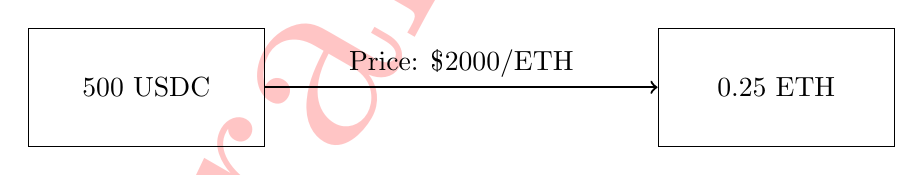
\begin{tikzpicture}[node distance=3cm, auto]

    % USD to ETH transaction
    \node (usdc) [rectangle, draw, text centered, minimum height=1.5cm, minimum width=3cm] {500 USDC};
    \node (eth) [rectangle, draw, right of=usdc, xshift=5cm, text centered, minimum height=1.5cm, minimum width=3cm] {0.25 ETH};

    % Arrow between them
    \draw[->, thick] (usdc) -- (eth) node[midway, above] {Price: \$2000/ETH};

\end{tikzpicture}

\newpage

\subsubsection{Step 2: Second Trade – Partial ETH to LINK}

After buying 0.25 ETH, the trader uses 0.1 ETH to buy LINK at the rate of \$7/LINK.

The USD/ETH trade is now partially closed with 0.15 ETH still held in the trader's account. A new ETH/LINK trade opens with 0.1 ETH used to buy LINK.

\begin{center}
  \scriptsize % Reduce font size
  \begin{longtable}{|p{0.8cm}|p{1.2cm}|p{1.5cm}|p{1.5cm}|p{1cm}|p{1.5cm}|p{1.5cm}|p{1cm}|p{1.5cm}|p{1.5cm}|}
    \hline
    \textbf{Trade ID} & \textbf{Pair} & \textbf{Entry Asset} & \textbf{Exit Asset} & \textbf{Amount} & \textbf{Price at Entry} & \textbf{Price at Exit} & \textbf{Status} & \textbf{Profit/Loss} & \textbf{Timestamp} \\
    \hline
    1 & USD/ETH & USD & ETH & 0.15 ETH & \$2000/ETH & N/A & Open & N/A & 2024-10-11 10:30:00 UTC \\
    \hline
    2 & ETH/LINK & ETH & LINK & 0.1 ETH & \$2000/ETH & \$7/LINK & Open & N/A & 2024-10-11 11:00:00 UTC \\
    \hline
    \caption{Trade Sheet After Second Trade}
    \end{longtable}
    \end{center}

The USD/ETH trade has been updated to show 0.15 ETH still open. A new ETH/LINK trade has opened with 0.1 ETH used to buy LINK.

\subsubsection*{Diagram for Second Trade}

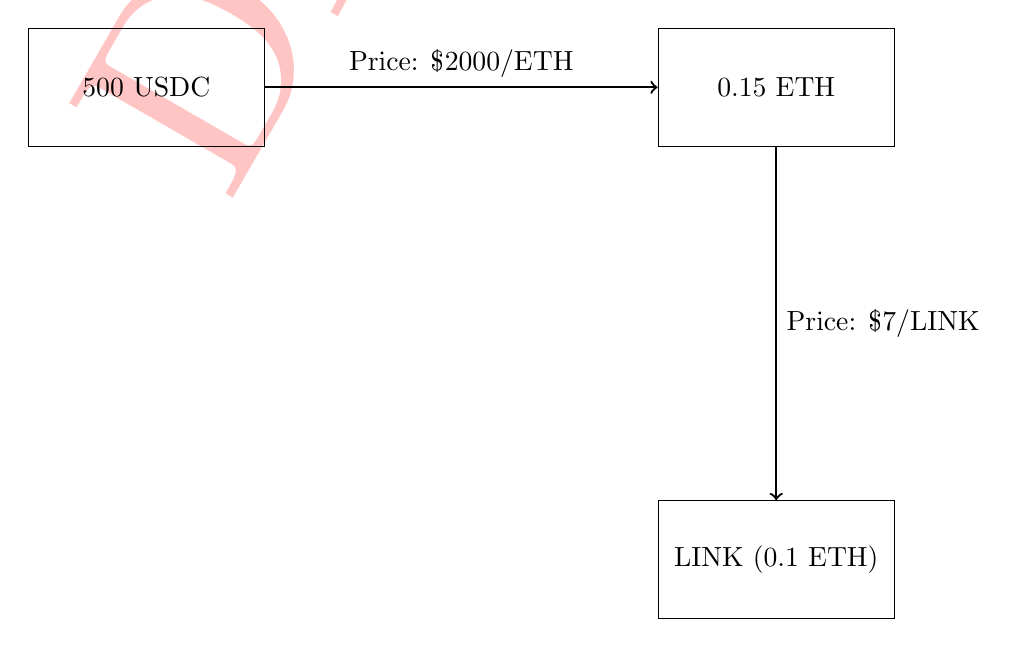
\begin{tikzpicture}[node distance=3cm, auto]

    % USD to ETH transaction (remaining ETH)
    \node (usdc) [rectangle, draw, text centered, minimum height=1.5cm, minimum width=3cm] {500 USDC};
    \node (eth) [rectangle, draw, right of=usdc, xshift=5cm, text centered, minimum height=1.5cm, minimum width=3cm] {0.15 ETH};

    % ETH to LINK transaction
    \node (link) [rectangle, draw, below of=eth, yshift=-3cm, minimum height=1.5cm, minimum width=3cm] {LINK (0.1 ETH)};

    % Arrows between them
    \draw[->, thick] (usdc) -- (eth) node[midway, above] {Price: \$2000/ETH};
    \draw[->, thick] (eth) -- (link) node[midway, right] {Price: \$7/LINK};

\end{tikzpicture}

\newpage

\subsubsection{PnL Calculations for the Second Trade}

Let’s calculate the profit or loss (PnL) for the second trade where 0.1 ETH was used to buy LINK.

\begin{align*}
\text{Entry Price of ETH} &= \$2000/ETH \\
\text{Exit Price of ETH} &= \$2200/ETH \text{ (for the portion used to buy LINK)} \\
\text{Amount Sold} &= 0.1 \text{ ETH}
\end{align*}

\[
\text{PnL} = (\text{Exit Price} - \text{Entry Price}) \times \text{Amount Sold}
\]
\[
\text{PnL} = (2200 - 2000) \times 0.1 = 200 \times 0.1 = \$20
\]

Thus, the realized profit for selling 0.1 ETH to buy LINK is \$20.

\subsubsection{Final Trade Sheet}

The trade sheet, with updated PnL for the closed portion, will look like this:

\begin{center}
  \scriptsize % Reduce font size
  \begin{longtable}{|p{0.8cm}|p{1.2cm}|p{1.5cm}|p{1.5cm}|p{1cm}|p{1.5cm}|p{1.5cm}|p{1cm}|p{1.5cm}|p{1.5cm}|}
  \hline
  \textbf{Trade ID} & \textbf{Pair} & \textbf{Entry Asset} & \textbf{Exit Asset} & \textbf{Amount} & \textbf{Price at Entry} & \textbf{Price at Exit} & \textbf{Status} & \textbf{Profit/Loss} & \textbf{Timestamp} \\
  \hline
  1 & USD/ETH & USD & ETH & 0.15 ETH & \$2000/ETH & N/A & Open & N/A & 2024-10-11 10:30:00 UTC \\
  \hline
  2 & ETH/LINK & ETH & LINK & 0.1 ETH & \$2000/ETH & \$2200/ETH & Closed & \$20 & 2024-10-11 11:00:00 UTC \\
  \hline
  \caption{Final Trade Sheet with PnL}
  \end{longtable}
  \end{center}
\subsection{Blockchain Data Analysis}
Explain the core technologies behind real-time wallet tracking, asset performance, and more.

\section{Technology Stack}
\subsection{Analytical Metrics}
Discuss the analytical metrics (e.g., wallet activity, asset performance, trade metrics) and how they assist in making smarter trading decisions.

\section{Tokenomics}
Explain the token model, distribution, and its role in the ecosystem.

\section{Roadmap}
Provide a roadmap for platform development and token launch.

\section{Team}
Introduce the team members and their expertise.

\section{Conclusion}
Summarize the impact of Aarkus Intelligence and the call to action for investors or partners.

\bibliographystyle{plain}  % You can use other styles like "unsrt", "ieeetr", etc.
\bibliography{references}  % This will reference the 'references.bib' file

\end{document}
